% DPF 09 talk on strangeness in nucleon

\documentclass[10pt]{beamer}
\usepackage{amsmath}
\usepackage{mathtools}
\usefonttheme{professionalfonts}
\usefonttheme{serif}
%\documentclass[12pt]{beamerthemeSam.sty}
\usepackage{epsf}
%\usepackage{pstricks}
%\usepackage[orientation=portrait,size=A4]{beamerposter}
\geometry{paperwidth=160mm,paperheight=120mm}
%DT favorite definitions
\def\LL{\left\langle}	% left angle bracket
\def\RR{\right\rangle}	% right angle bracket
\def\LP{\left(}		% left parenthesis
\def\RP{\right)}	% right parenthesis
\def\LB{\left\{}	% left curly bracket
\def\RB{\right\}}	% right curly bracket
\def\PAR#1#2{ {{\partial #1}\over{\partial #2}} }
\def\PARTWO#1#2{ {{\partial^2 #1}\over{\partial #2}^2} }
\def\PARTWOMIX#1#2#3{ {{\partial^2 #1}\over{\partial #2 \partial #3}} }

\def\rightpartial{{\overrightarrow\partial}}
\def\leftpartial{{\overleftarrow\partial}}
\def\diffpartial{\buildrel\leftrightarrow\over\partial}

\def\BI{\begin{itemize}}
\def\EI{\end{itemize}}
\def\BE{\begin{displaymath}}
\def\EE{\end{displaymath}}
\def\BEA{\begin{eqnarray*}}
\def\EEA{\end{eqnarray*}}
\def\BNEA{\begin{eqnarray}}
\def\ENEA{\end{eqnarray}}
\def\EL{\nonumber\\}


\newcommand{\map}[1]{\frame{\frametitle{\textbf{Course map}}
\centerline{\includegraphics[height=0.86\paperheight]{../../map/#1.png}}}}
\newcommand{\wmap}[1]{\frame{\frametitle{\textbf{Course map}}
\centerline{\includegraphics[width=0.96\paperwidth]{../../map/#1.png}}}}

\newcommand{\etal}{{\it et al.}}
\newcommand{\gbeta}{6/g^2}
\newcommand{\la}[1]{\label{#1}}
\newcommand{\ie}{{\em i.e.\ }}
\newcommand{\eg}{{\em e.\,g.\ }}
\newcommand{\cf}{cf.\ }
\newcommand{\etc}{etc.\ }
\newcommand{\atantwo}{{\rm atan2}}
\newcommand{\Tr}{{\rm Tr}}
\newcommand{\dt}{\Delta t}
\newcommand{\op}{{\cal O}}
\newcommand{\msbar}{{\overline{\rm MS}}}
\def\chpt{\raise0.4ex\hbox{$\chi$}PT}
\def\schpt{S\raise0.4ex\hbox{$\chi$}PT}
\def\MeV{{\rm Me\!V}}
\def\GeV{{\rm Ge\!V}}

%AB: my color definitions
%\definecolor{mygarnet}{rgb}{0.445,0.184,0.215}
%\definecolor{mygold}{rgb}{0.848,0.848,0.098}
%\definecolor{myg2g}{rgb}{0.647,0.316,0.157}
\definecolor{abtitlecolor}{rgb}{0.0,0.255,0.494}
\definecolor{absecondarycolor}{rgb}{0.0,0.416,0.804}
\definecolor{abprimarycolor}{rgb}{1.0,0.686,0.0}
\definecolor{Red}           {cmyk}{0,1,1,0}
\definecolor{Grey}           {cmyk}{.7,.7,.7,0}
\definecolor{Lg}           {cmyk}{.4,.4,.4,0}
\definecolor{Blue}          {cmyk}{1,1,0,0}
\definecolor{Green}         {cmyk}{1,0,1,0}
\definecolor{Brown}         {cmyk}{0,0.81,1,0.60}
\definecolor{Black}         {cmyk}{0,0,0,1}

\usetheme{Madrid}


%AB: redefinition of beamer colors
%\setbeamercolor{palette tertiary}{fg=white,bg=mygarnet}
%\setbeamercolor{palette secondary}{fg=white,bg=myg2g}
%\setbeamercolor{palette primary}{fg=black,bg=mygold}
\setbeamercolor{title}{fg=abtitlecolor}
\setbeamercolor{frametitle}{fg=abtitlecolor}
\setbeamercolor{palette tertiary}{fg=white,bg=abtitlecolor}
\setbeamercolor{palette secondary}{fg=white,bg=absecondarycolor}
\setbeamercolor{palette primary}{fg=black,bg=abprimarycolor}
\setbeamercolor{structure}{fg=abtitlecolor}

\setbeamerfont{section in toc}{series=\bfseries}

%AB: remove navigation icons
\beamertemplatenavigationsymbolsempty
\title[Work and potential energy]{
  \textbf {Work and potential energy}\\
%\centerline{}
%\centering
%\vspace{-0.0in}
%\includegraphics[width=0.3\textwidth]{propvalues_0093.pdf}
%\vspace{-0.3in}\\
%\label{intrograph}
}

\author[W. Freeman] {Physics 211\\Syracuse University, Physics 211 Spring 2022\\Walter Freeman}

\date{\today}

\begin{document}

\frame{\titlepage}


\frame{\frametitle{\textbf{Announcements}}
	
\BI
\item I didn't get the weekly Google Form sent out last week (sorry)
\item I am going to grade these differently than planned:
\BI
\item Completing them will help your grade
\item Not completing them won't hurt your grade
\EI
\vspace{.4in}


\item Homework 6 due date postponed until Friday (we're covering one topic today)
\item Homework 7 will be assigned tomorrow and will be due the following Friday -- it will be long
\EI

\vspace{.4in}

My help hours this week in the Physics Clinic:

\BI
\item Tuesday, 9:45-10:45 AM and 2-3:45 PM
\item Wednesday, 2:30-3:30 PM
\item Thursday, 9:45-10:45 AM and 2:30-3:30 PM
\EI




}	

\frame{\frametitle{\textbf{Ask the Physicist: nuclear energy}}

Basic nuclear chemistry:

\BI
\item Atomic nuclei are made of protons and neutrons
\item The element name tells you how many protons; the number is the sum of protons+neutrons
\item The element name (proton number) determines its {\it chemical} properties
\item Both proton and neutron number determine {\it nuclear} properties
\item Examples:
\BI

{\color{Red}\item Carbon-12 (6 protons, 6 neutrons) is chemically the same as carbon-14 (6 protons, 8 neutrons)
\item Carbon-12 is stable; carbon-14 is radioactive (decays slowly over time)

\bigskip
}
{\color{Green}
\item Uranium-238 (99.4\% of natural uranium) and uranium-235 (the rest)

}
\EI

\bigskip

\item Elements with the same proton number (name) but different neutron number are called {\it isotopes}
\item They cannot be separated chemically and occur together

\EI
}


\frame{\frametitle{\textbf{Radioactivity and potential energy -- unrelated!}}
	
	Some isotopes are {\it radioactive} and decay (transform) into other elements over a period of time, producing
	another nucleus plus a fast-moving particle with a lot of kinetic energy:
	
	\bigskip
	
	This cannot be used as a primary energy source: 
	
	\BI
	\item Anything that decays quickly isn't found in nature
	\item Anything that decays slowly releases energy too slowly
	\pause
	\item \color{Blue} Radioactivity has little to do with nuclear power (rare exceptions: spacecraft, old pacemakers)
	\EI
	
	{\color{Red} \pause}
	
	\bigskip\bigskip
	
	\begin{minipage}{0.5\textwidth}
		\color{Red}
		
	But there {\it is} a lot of potential energy in nuclei. 
	
	\bigskip
	
	This graph is of {\it inverse} potential energy.
	\bigskip
	
	The units on the vertical axis are roughly equivalent to ``hundred trillion joules per kilogram''
	    \end{minipage}
	\begin{minipage}{0.45\textwidth}
	\begin{center}
		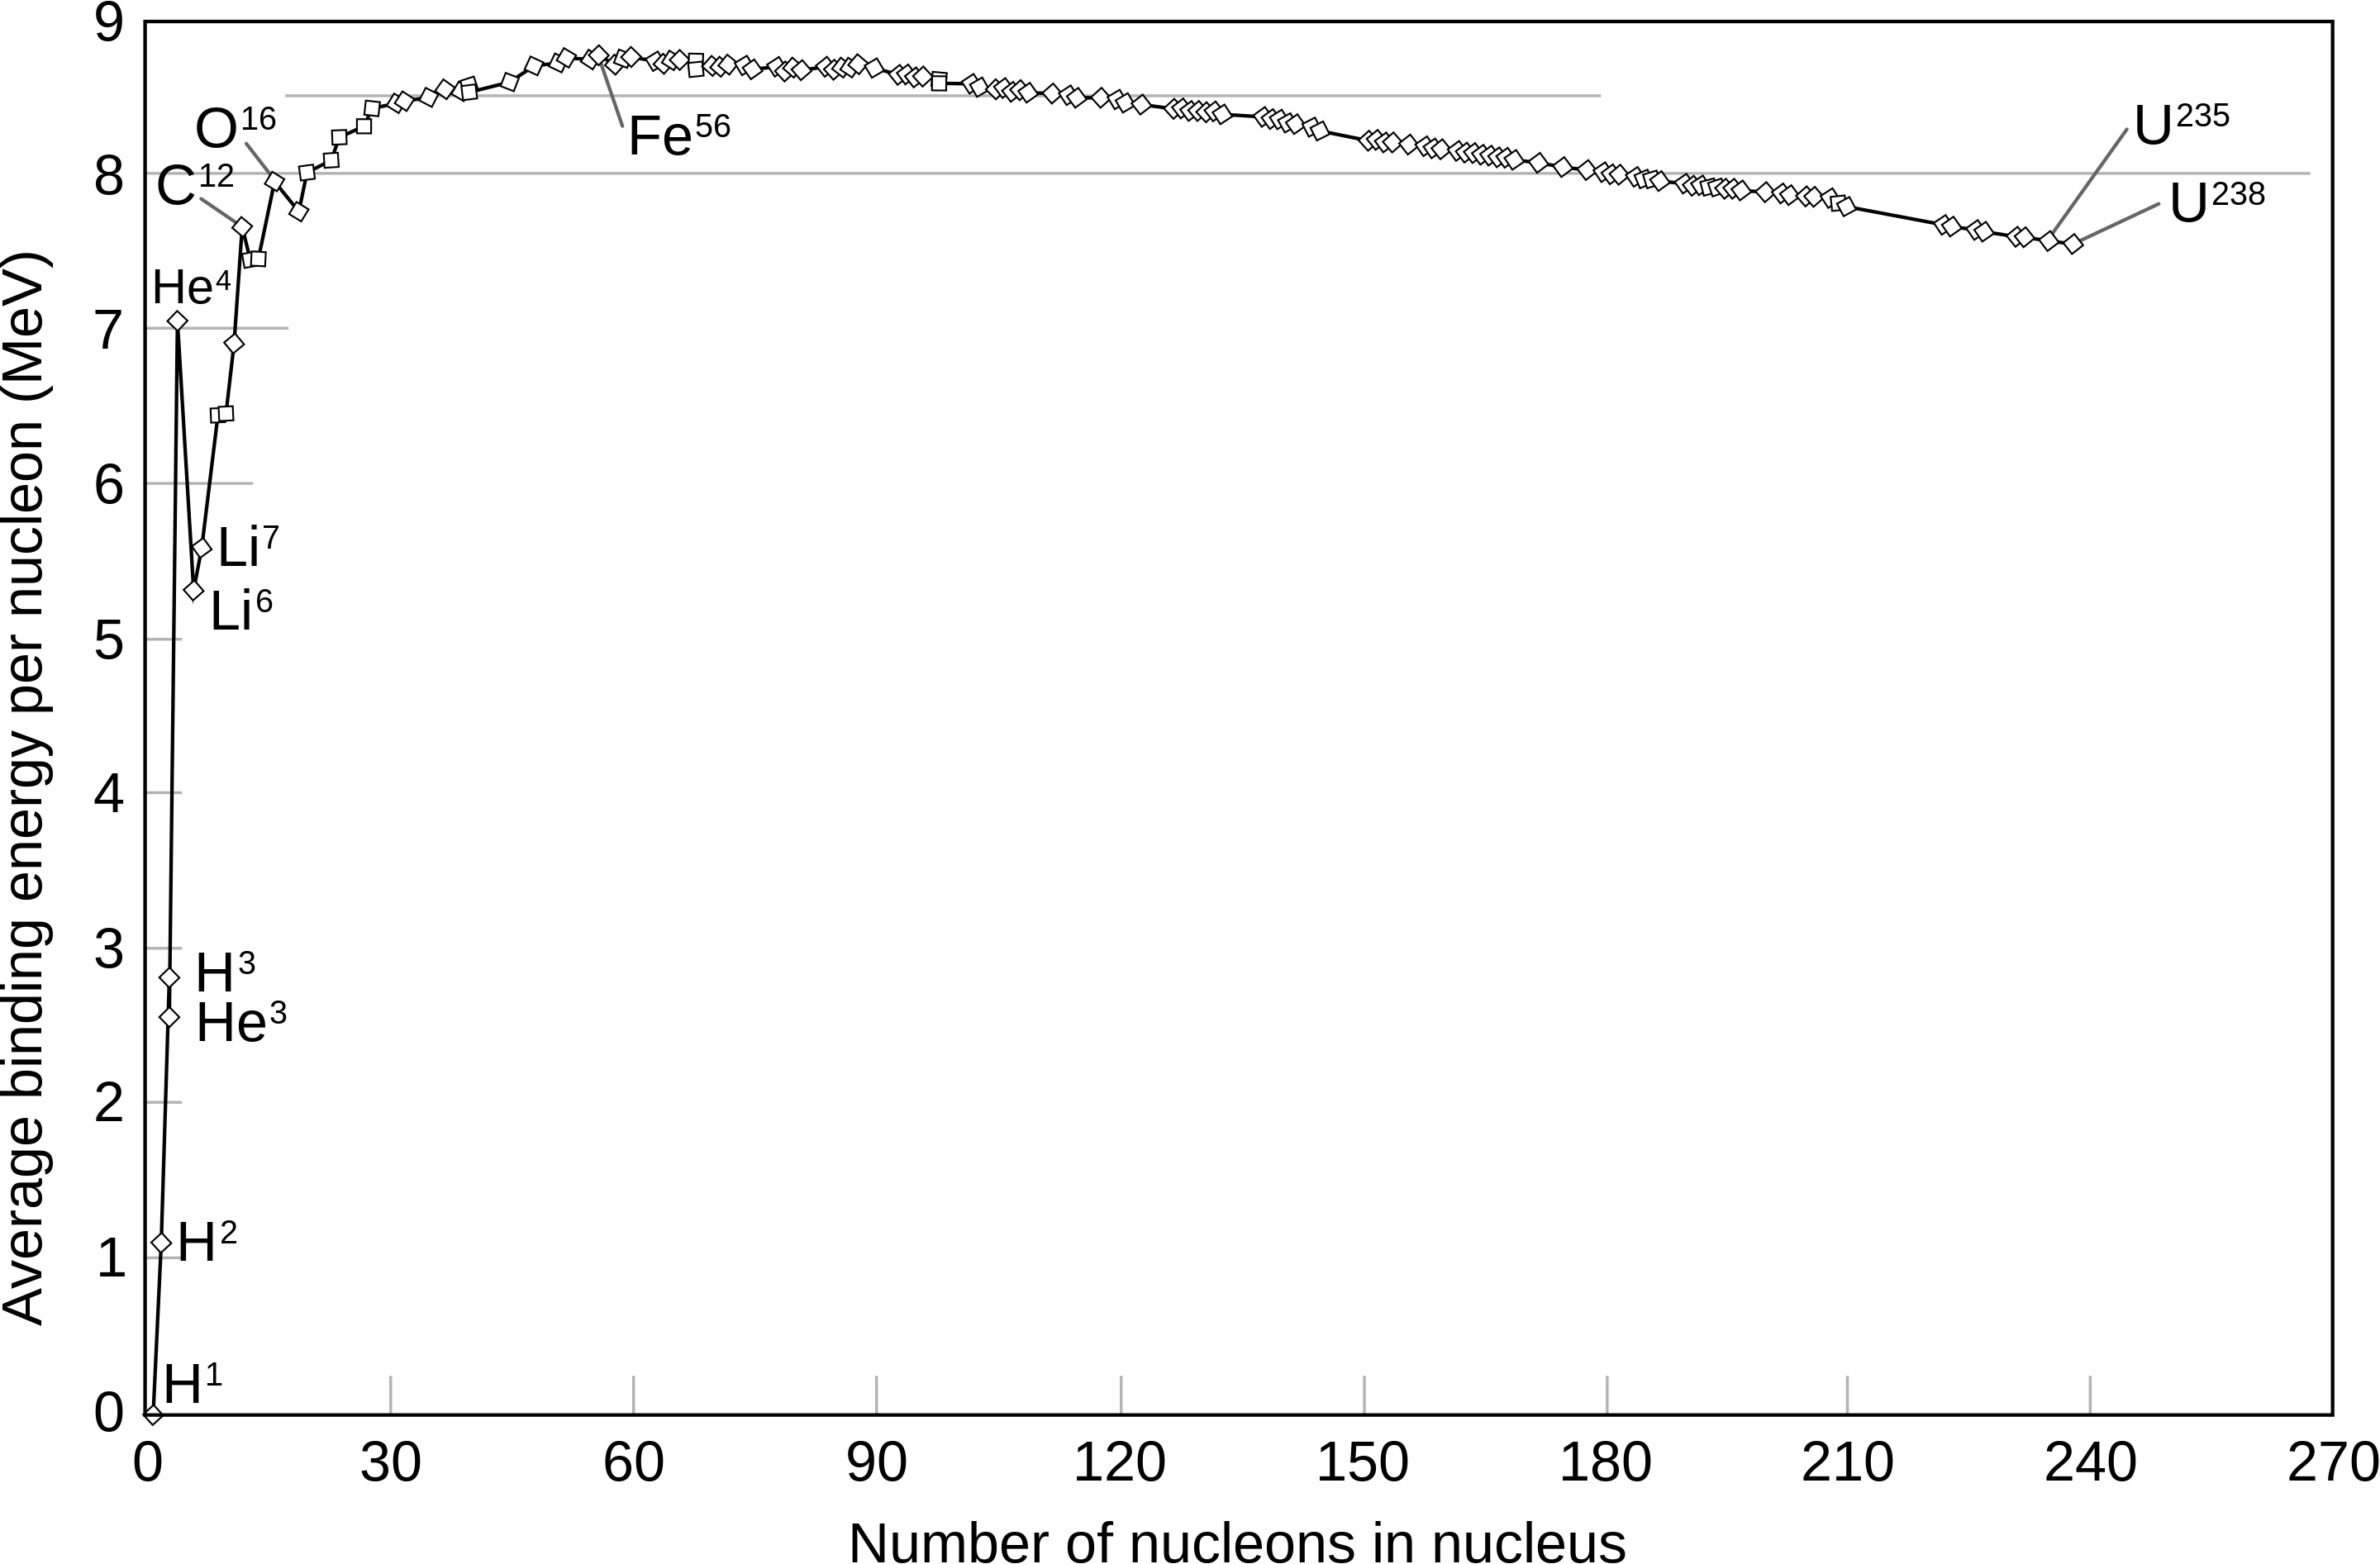
\includegraphics[width=0.9\textwidth]{binding-energy.png}
	\end{center}
    \end{minipage}

\color{Green}
How can we harness this energy?
}

\frame{

\begin{center}
	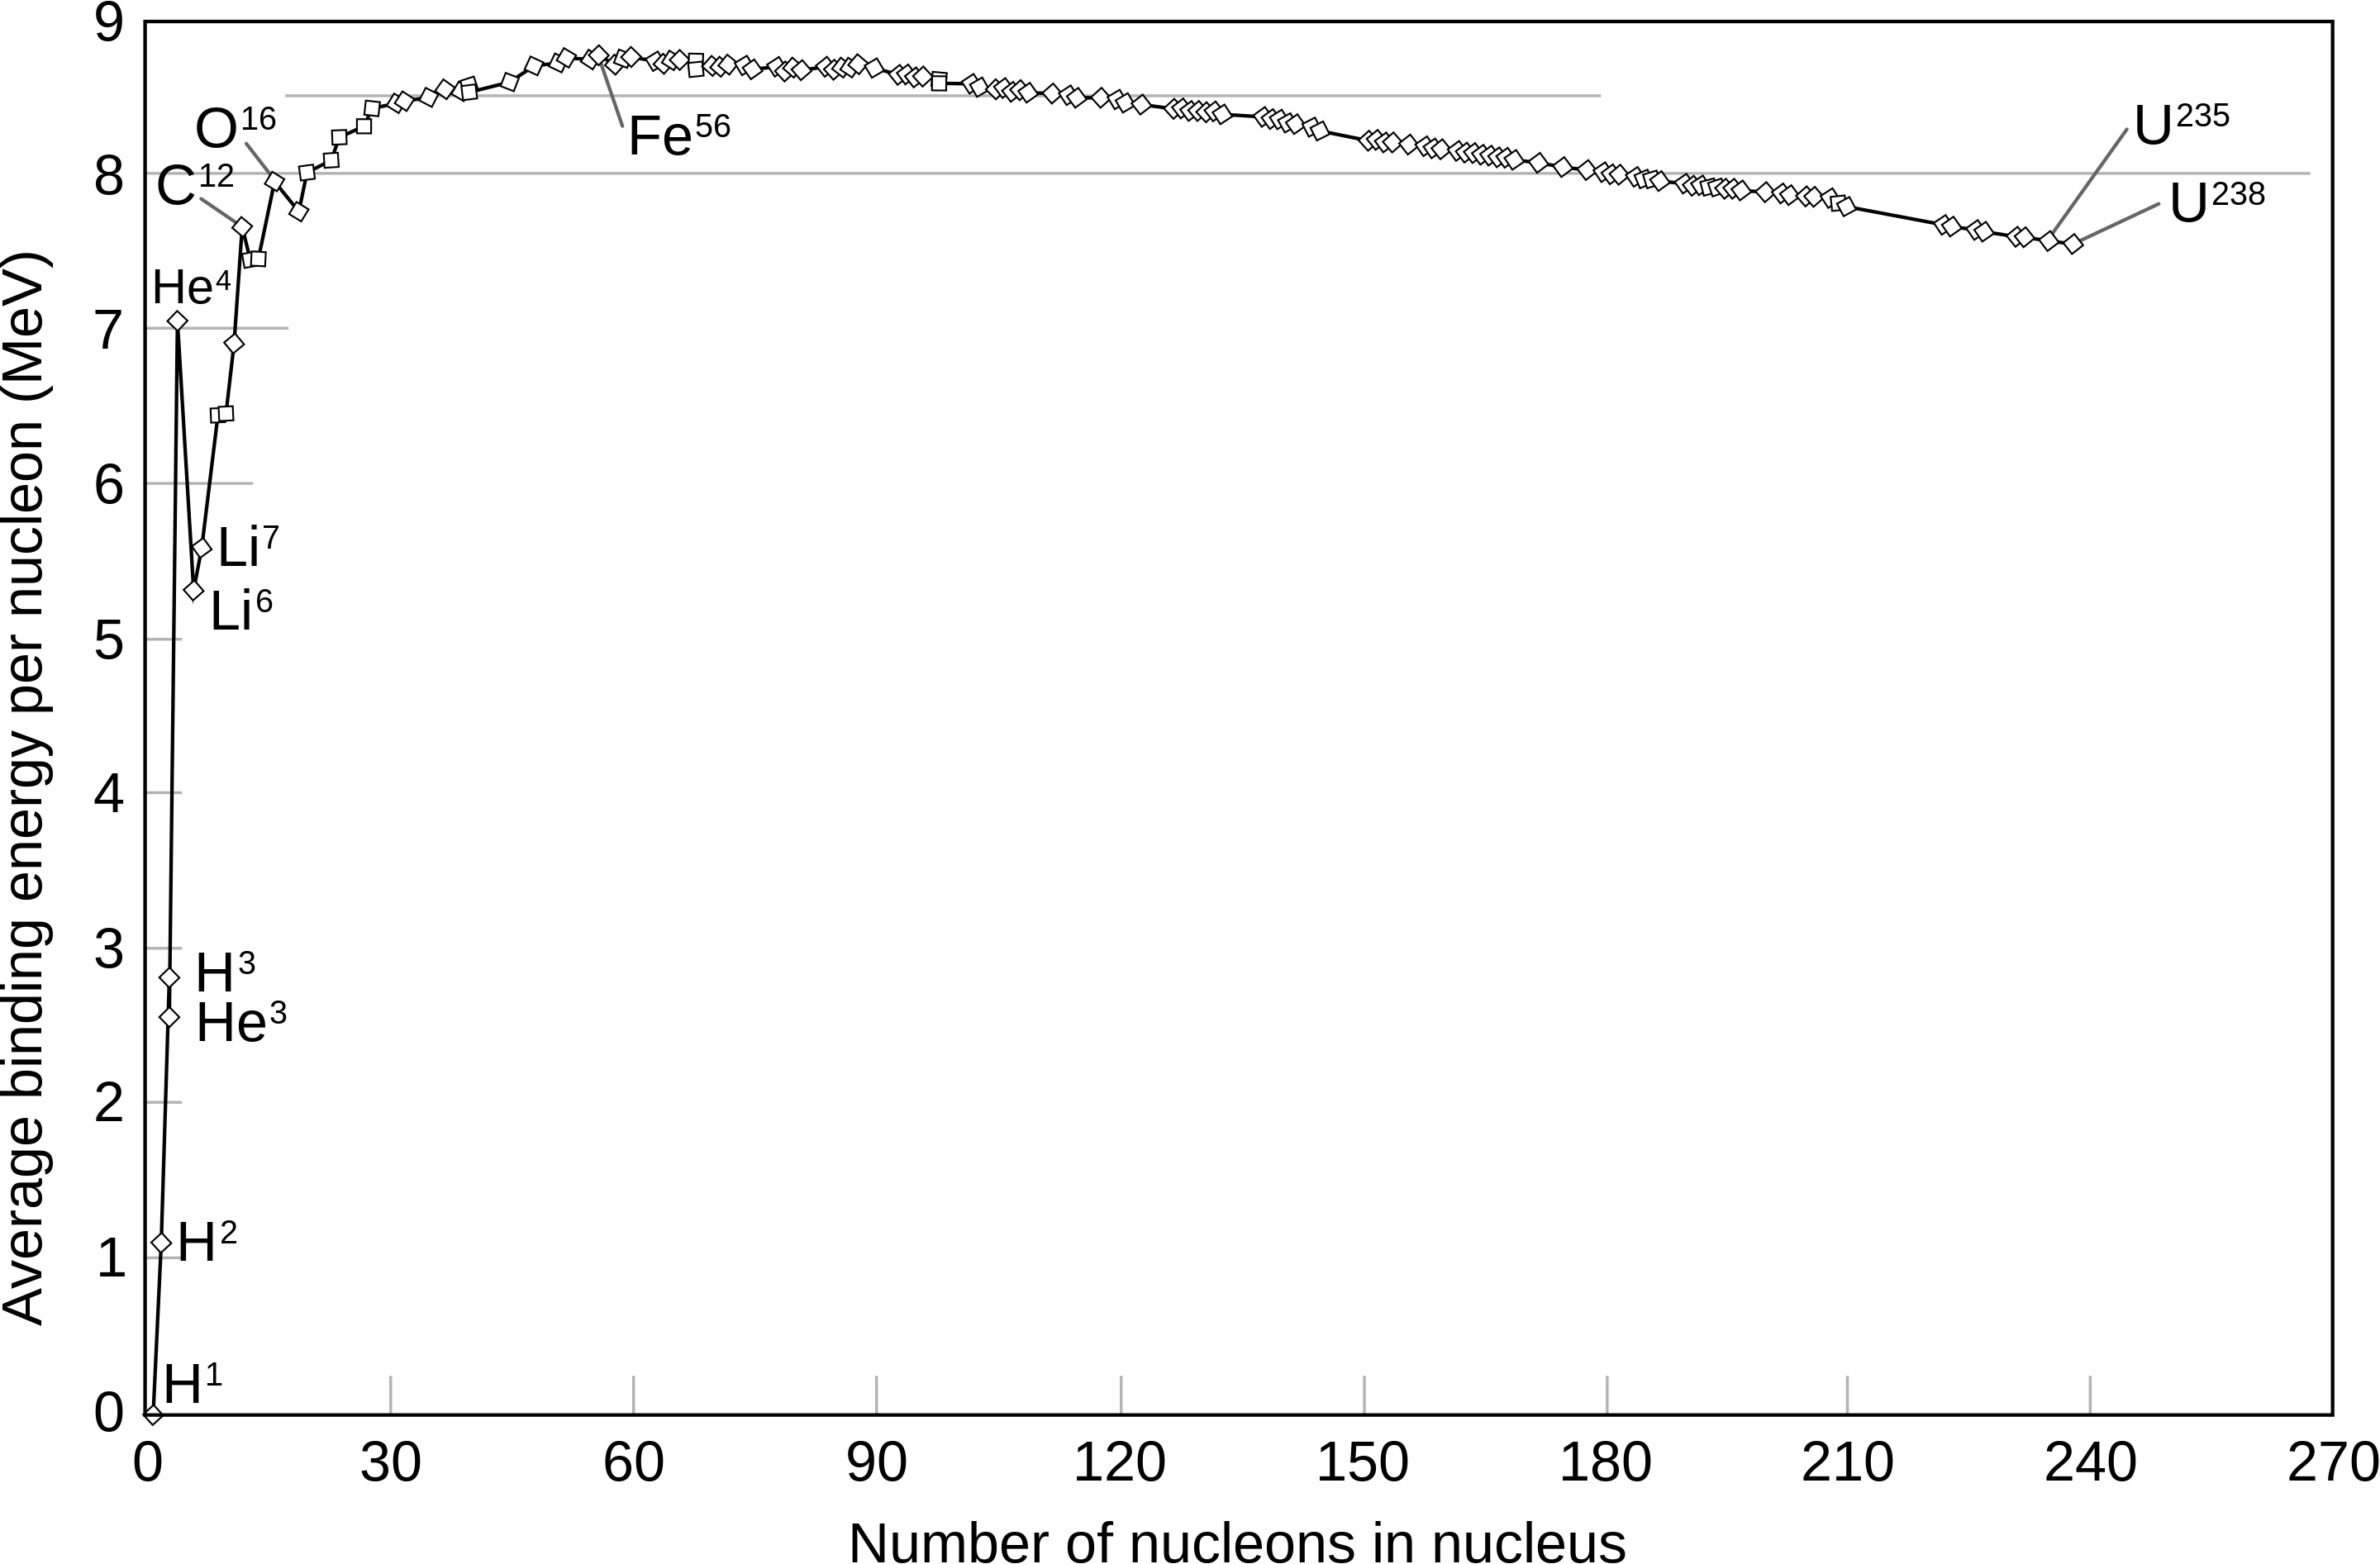
\includegraphics[width=0.6\textwidth]{binding-energy.png}	
\end{center}

\begin{itemize}
	\item Fusion: stick little nuclei together to make big ones
	\BI
		\item Requires incredibly high temperatures (hard for us, easy for stars)
		\item Not practical on Earth (yet)
		\EI
\end{itemize}


\begin{itemize}
	\item Fission: split apart big nuclei to make smaller ones
	\BI
	\item Only a few nuclei are {\it fissile} (can be split)
	\item The only naturally-occurring one is $\null^{235}\rm U$ (0.6\%)
	\item It's hard to separate from $\null^{238}\rm U$ (99.4\%)
	\EI
\end{itemize}
}



\frame{\frametitle{\textbf{Nuclear fission}}
	We got lucky:
	
	\begin{enumerate}
		\item 	$\null^{235}\rm U$ nuclei split into two pieces when struck by a neutron \pause
		\item This produces a lot of energy \pause
		\item ... this also produces 2-3 more neutrons \pause
		\item {\color{Red} $\rightarrow$ ... chain reaction!}
	\end{enumerate}

\bigskip


But there's a complication:

\begin{enumerate}
	\item $\null^{238}\rm U$ nuclei tend to absorb neutrons and don't fission
	\item The neutrons produced by the fission reaction are ``fast''
	\item ``Slow'' neutrons are more likely to induce fission in 	$\null^{235}\rm U$ nuclei
\end{enumerate}\pause

\bigskip

We thus need to protect the neutrons from getting eaten by 	$\null^{238}\rm U$ while slowing them down with a {\it moderator}. Two approaches:

\begin{enumerate}
	\item Really efficient moderator and natural (0.6\% 	$\null^{235}\rm U$) uranium
	\BI
	\item Graphite moderated, water cooled -- old Soviet (RBMK)
	\item Heavy water moderated and cooled -- Canadian (CANDU)
	\EI
	\item Less efficient moderator and enriched uranium
	\BI
	\item Take some of the 	$\null^{238}\rm U$ out so it stops eating neutrons
	\item Light water moderated, light water cooled -- everyone else
	\EI
\end{enumerate}

Enormous amount of energy: 1 gigawatt for two months per ton of uranium
}




	
	
\frame{\frametitle{\textbf{A new force: elasticity and Hooke's law}}
To best see how this can be useful, let's introduce a new force: elasticity.

\begin{itemize}

  \item{Springs have a particular length that they like to be: ``equilibrium length'' $L_0$}
  \item{A spring stretched to be longer than this pulls inward to shorten itself}
  \item{A spring compressed to be shorter than this pushes outward to lengthen itself}
  \item{Flexible things like strings and ropes only pull; they kink instead of compressing}
  \item{The force is proportional to the deviation from the optimum length}
\EI
\centerline{    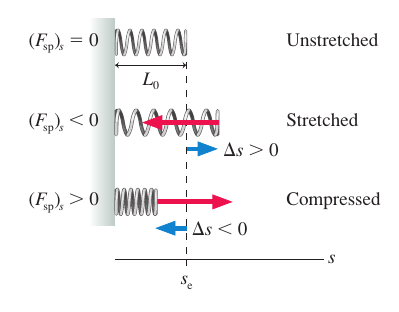
\includegraphics[width=0.4\textwidth]{hooke.png}}
\Large
\centerline{$F_{\rm{elastic}} = -k (L - L_0) = -k \Delta x$ (Hooke's law)}

\bigskip
\pause
\large
$k$ is called the ``spring constant'':

\BI
\item{Measures the stiffness of the spring/rope}
\item{Units of newtons per meter: ``restoring force of $k$ newtons per meter of stretch''}
  \EI
}


\frame{\frametitle{\textbf{A simple spring problem: done with the work-energy theorem}}
\Large
A person of mass $m=100 kg$ falls from a height of $h=3$m onto a trampoline. If the person makes an impression $d=40$ cm deep on the trampoline when he lands, what is the spring constant?

\pause
\bigskip
\bigskip
\bigskip

\normalsize

\BI
\item{Initial kinetic energy + work done by spring + work done by gravity = final kinetic energy}
  \BI
\item{Need to use the integral form of the work-energy theorem since the force isn't constant}
  \EI
\item{The person begins and ends at rest, so we know the initial and final kinetic energy is zero}
\item{The trampoline begins at its equilibrium position}
  \pause
\item{\color{Red}$W_{\rm{grav}} = (mg)(h+d)$}
  \pause
\item{\color{Blue}$W_{\rm{elas}} = \int_0^{-d} \, kx \, dx = -\frac{1}{2} kd^2$}
  \pause
\item{$KE_0 + {\color{Red}W_{\rm{grav}}} + {\color{Blue}W_{\rm{elas}}} = KE_f$}
\item{$0 + \color{Red}(mg)(h+d) \color{Blue}-\frac{1}{2} kd^2 \color{Black}= 0$}
\item{$k = \frac{mg(h+d)}{2d^2}$}
  \EI
}
  

\frame{\frametitle{\textbf{Potential energy stored in a spring}}
\Large 
We saw that an object at height $h$ has gravitational potential energy $mgh$. Can we do something similar for springs?

\large

\bigskip
\bigskip
\pause
\BI
\item{Potential energy, remember, is the work done by some force as it returns to some ``zero'' position.}
\item{A natural choice is $\Delta x=0$, the equilibrium position of the spring.}
  \EI

\Large

``How much work is done by a spring as it goes from $\Delta x=a$ to $\Delta x=0$?

\bigskip
\bigskip

\centerline{$U_{\rm{elastic}} = W_{a \rightarrow 0} = \int_a^0 \, -kx \, dx = \int_0^a \, kx \, dx = \frac{1}{2}ka^2$}

\pause
\bigskip
\bigskip

Now that we have this, we never have to do this integral again!

\bigskip

\centerline{$U_{\rm{elastic}} = \frac{1}{2} kx^2$, where $x$ is the distance from equilibrium}

}


  
  
   
  \frame{\frametitle{\textbf{A simple spring problem: done with potential energy}}
\Large
A person of mass $m=100$ kg falls from a height of $h=3$m onto a trampoline. If the person makes an impression $d=40$ cm deep on the trampoline when he lands, what is the spring constant?

\pause
\bigskip
\bigskip
\bigskip

\normalsize

\BI
\item{Initial total energy + work done by other forces = final total energy}
\item{We have no ``other forces'': we're accounting for gravity and elasticity using potential energy}
\item{The person begins and ends at rest, so we know the initial and final kinetic energy is zero}
\item{Put $y=0$ at the surface of the trampoline}
  \pause
\item{$U_{\rm{grav},0} = mgh$}
\item{$U_{\rm{elas},0} = 0$ (trampoline starts at equilibrium)}
\item{$U_{\rm{grav},f} = -mgd$ (the person falls below $y=0$; PE can be negative!)}
\item{$U_{\rm{elas},f} = \frac{1}{2}kd^2$ (see last slide)}
  \pause
\item{${\color{Lg}KE_0} + U_{\rm{grav},0} + {\color{Lg}U_{\rm{elas},0}} = {\color{Lg}KE_f} + U_{\rm{grav},f} + U_{\rm{elas},f}$}
  \pause
\item{$0 + mgh + 0 = 0 + (-mgd) + \frac{1}{2}kd^2$ (Same terms, maybe on different side)}
  \pause
\item{$k = \frac{mg(h+d)}{2d^2}$}
  \EI
}
  \frame{\frametitle{\textbf{That spring problem: a recap}}
     \large
     \centerline{We don't care about time $\rightarrow$ energy methods}

     \bigskip
     \normalsize

     \begin{columns}
     \column{0.5\textwidth}
     \centerline{Work-energy theorem}
     \column{0.5\textwidth}
     \centerline{Potential energy treatment}
   \end{columns}
   \begin{columns}
     \column{0.5\textwidth}

     \BI
   \item{Initial KE + all work done = final KE}
   \item{Need to compute work done by gravity: easy}
   \item{Need to compute work done by spring: harder\\(need to integrate Hooke's law)}
   \EI
   \column{0.5\textwidth}
   \BI
 \item{Initial KE + initial PE + other work = final KE + final PE}
 \item{No ``other work'' in this problem; all forces have a PE associated}
 \item{Need to know the expressions for PE:}
   \BI
 \item{$U_{\rm{grav}} = mgy$}
 \item{$U_{\rm{elas}} = \frac{1}{2}kx^2$ (x is the distance from the equilibrium point)}
   \EI
 \item{No integrals required (they're baked into the above)}
   \EI
 \end{columns}
 }

 \frame{\frametitle{\textbf{Potential energy with other forces}}
   \large
   What about associating a potential energy with other forces?\normalsize
   \BI
 \item{Friction is a no-go: the work done by friction depends on the path, not just where you start and stop}
 \item{``Ephemeral'' forces like tension and normal force are easiest to deal with by computing work directly}
% \item{The other force we've studied that is easily associated with a potential energy is {\bf universal gravitation}}
%   \BI
% \item{Need to choose a point to set $U=0$; here we choose $r = \infty$}
% \item{$U_G$ = ``work done by gravity on $m_1$ when it moves infinitely far from $m_2$}
%   \EI
\EI
%
%\bigskip
%\bigskip
%
%\Large
%
%   $F_G = \frac{Gm_1 m_2}{r^2}$
%   
%\bigskip
%
%   $W_G = \int_R^\infty\, -\frac{Gm_1m_2}{r^2}\, dr = -\frac{Gm_1 m_2}{R}$
%
%   \pause
%   \bigskip
%
%   $\rightarrow$ Gravitational potential energy between two objects separated by a distance $r$ is $-\frac{Gm_1m_2}{r}$.
 }
%
% \frame{\frametitle{\textbf{The Earth's ``gravity well''}}
%   \large
%    \BI
%  \item{With this choice of the zero point at $r=\infty$, gravitational potential energy is always negative}
%  \item{We have to {\it add energy} to get something away from Earth}
%\EI  
%\bigskip
%
%\centerline{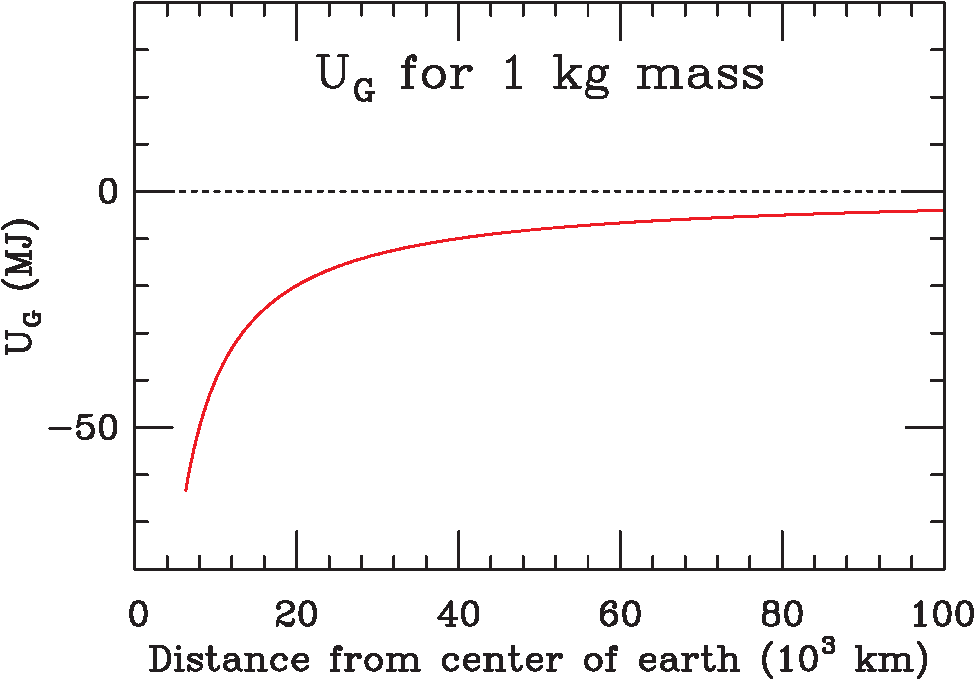
\includegraphics[width=0.6\textwidth]{ug-crop.pdf}}
%
%\bigskip
%
%This region of large negative potential energy is often called a ``gravity well''.
%}


\frame{\frametitle{\textbf{Problem-solving guide for problems involving energy}}
	\large
	\BI
	\item Identify the various parts of the motion and what you need to know about them
	\BI
	%	\item Collisions/explosions: use conservation of momentum
	\item Motion where you care only about begin/end states and not time: use work/energy methods
	\item ``Where does it land'' projectile motion problems: can {\color{Red}not} use energy methods
	\EI
	\item Draw a series of snapshots, showing what your ``before'' and ``after'' pictures look like 
	(you may have more than two in some problems)
	\item Use force diagrams to calculate any forces you need to know
	\item Application of the work-energy theorem:
	\EI
	$$KE_{\rm initial} + W_{\rm all} = KE_{\rm final}$$
	
	\centerline{OR}
	
	$$KE_{\rm initial} + PE_{\rm initial} + W_{\rm other} = KE_{\rm final} + PE_{\rm final}$$
}


\frame{\frametitle{\textbf{Sample problems}}
	
	\Large
	A mass $m$ is hung from a spring of spring constant $k$ and released. Which equation 
	would let me find the distance $d$ that it falls before it comes back up?
	
	
	\BI
	\item A: $mgd - \frac{1}{2}kd^2 = 0$
	\item B: $\frac{1}{2}kx^2 = mgd + \frac{1}{2}mv^2$
	\item C: $0 = -mgd + \frac{1}{2}kd^2$
	\item D: $mgd + \frac{1}{2}kd^2 = 0$
	\EI
}

\frame{\frametitle{\textbf{Sample problems}}
	\large
	
	A spring is used to launch a block up a ramp of total length L. The spring has spring constant $k$, the block has mass $m$,
	the ramp is inclined an angle $\theta$, and it has a coefficient of kinetic friction $\mu_k$. 
	I compress the spring a distance $x$ and let it go. How fast will the block be traveling when it reaches 
	the top of the ramp?
	
	\bigskip\bigskip
	
	Which equation would let me solve for this?
	
	\BI
	\item A: $\frac{1}{2}kx^2 + \mu mgL \cos \theta = \frac{mgL}{\sin \theta} - \frac{1}{2}mv_f^2$
	\item B: $-\frac{1}{2}kx^2 + \mu mgL \sin \theta = \frac{mgL}{\sin \theta} + \frac{1}{2}mv_f^2$
	\item C: $\frac{1}{2}kx^2 - \mu mgL \sin \theta = mgL \cos \theta + \frac{1}{2}mv_f^2$
	\item D: $\frac{1}{2}kx^2 - \mu mgL \cos \theta = mgL \sin \theta + \frac{1}{2}mv_f^2$
	\EI
}

\frame{\frametitle{\textbf{Sample problems}}
	\Large
	A car coasts down a ramp and then up around a loop of radius $r$. How high must the ramp be for the car
	to make it around the loop? (See picture on document camera.)
	
	\bigskip
	
	How am I going to do this problem?
	\bigskip
	
	\large
	\BI
	\item A: Use conservation of momentum to relate the height of the ramp to the speed at the top of the loop,
	then use kinematics to determine if it will fall or not.
	\item B: Use conservation of energy to relate the height of the ramp to the speed at the top, then
	use kinematics to determine at what point it will fall in the loop.
	\item C: Use conservation of energy to relate the height of the ramp to the speed at the top, then
	use Newton's second law and our knowledge of rotational motion to determine the required speed.
	\item D: Use kinematics to relate the height of the ramp to the speed entering the loop, then
	use Newton's second law and our knowledge of rotational motion to determine the required speed.
	\EI
}


\frame{\frametitle{\textbf{Power: rate of doing work}}
	\large
	A bit of mathematics that will be useful to you:
	
	\bigskip
	
	{\bf ``An object moves at a constant speed $\vec v$, subject to some force $\vec F$; at what rate does that force do work on the object?''}
	
	\bigskip
	
	An example: an airplane flies at v=1000 m/s, and its engines exert F=300 kN of thrust. What is the rate at which the engines do work (power)?
	
	\bigskip
	
	\centerline{Work = force $\cdot$ distance}
	\pause
	\centerline{Power = work / time}
	\pause
	\centerline{Power = force $\cdot$ distance / time}
	\pause
	\centerline{Power = force $\cdot$ (distance / time)}
	\pause
	\centerline{Power = force $\cdot$ velocity}
	\pause
	\centerline{$P = \vec F \cdot \vec v = {\color{Red}300 MW}$}
	
	\bigskip
	
	\BI
	\item{The engines output 300 MW of power: this is around 10 liters per second of fuel even at 100\% efficiency!}
	\item{Some of that 300 MW of energy dissipated by drag heats up the airplane... (real numbers for a SR-71 Blackbird)}
	\EI
}



%\frame{\frametitle{\textbf{Sample problems}}
%	\Large
%	A truck pulling a heavy load with mass $m=4000$ kg wants to drive up a hill at a $30^\circ$ grade.
%	
%	\bigskip
%	\bigskip
%	
%	If the truck's engine can produce 100 kW of power (134 hp), how fast can the truck go? (Neglect drag.)
%	
%}

\frame{\frametitle{\textbf{Sample problems}}
	\Large
	A 1000 kg car has an engine that produces up to P=100 kW of power. If it accelerates as hard as it can, at what speed
	does its acceleration become limited by the engine? 
	
	\bigskip
	\bigskip
	\pause
	
	(What else would limit its acceleration?)
	
	\bigskip
	\bigskip
	\pause
	
	At low speeds: static friction limits acceleration\\
	At high speeds: engine power limits acceleration}



%\frame{\frametitle{\textbf{Sample problems}}
%	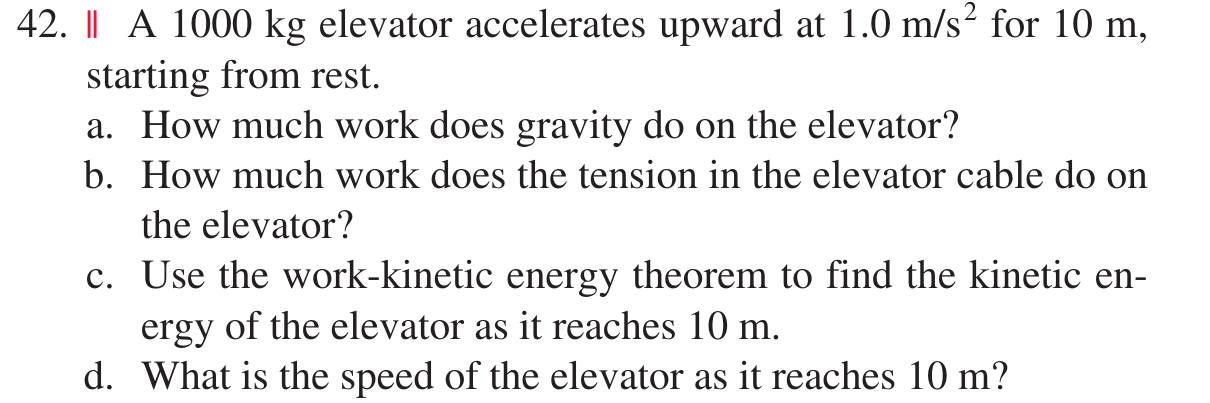
\includegraphics[width=0.7\textwidth]{elevator.png}
%}




\frame{\frametitle{\textbf{Sample problems}}
	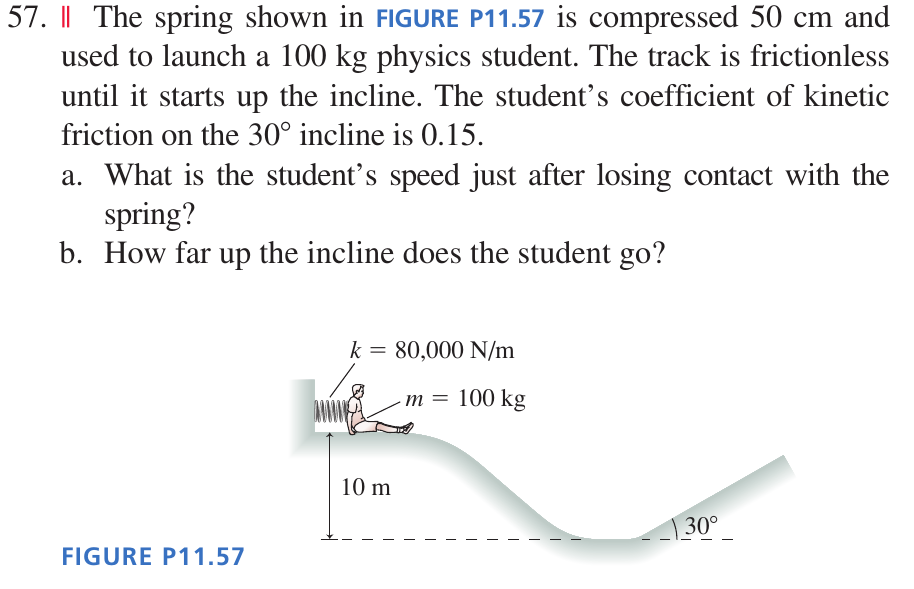
\includegraphics[width=0.7\textwidth]{student-on-spring.png}
}

\frame{\frametitle{\textbf{Sample problems}}
	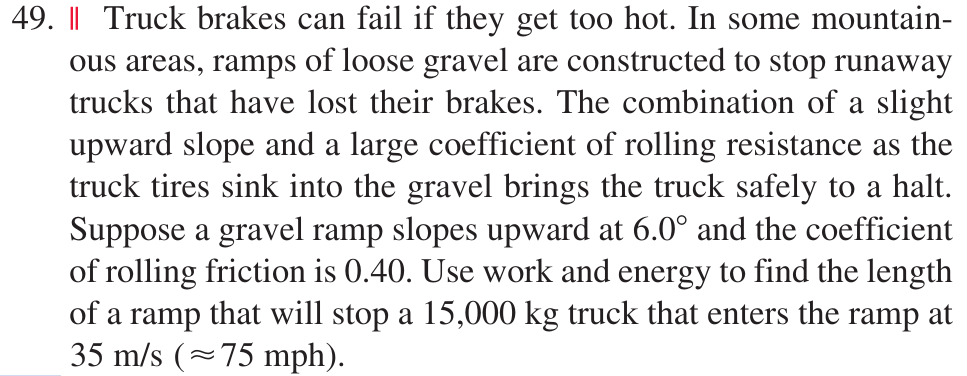
\includegraphics[width=0.7\textwidth]{runaway.png}
}


 \frame{\frametitle{\textbf{Summary}}
\large
   \BI
 \item{Potential energy is two things:}
   \BI
 \item{An accounting device that makes it easier to keep track of work done}
 \item{Part of {\it conservation of total energy}, a powerful statement about nature}
   \EI
 \item{Gravitational potential energy (on Earth): $U_g = mgy$}
   \pause
   
   \bigskip
 \item{We learned about a new force: {\bf elasticity}}
   \BI
 \item{Restoring force in a stretched or compressed spring, or a stretched string: }
   \large   \centerline{$F = -k(x-x_0)$ ($x_0$ is the equilibrium length)} \normalsize
 \item{$k$ is the spring constant, measured in force per distance, that gauges stiffness}
 \item{Elastic potential energy: $U_{\rm{elas}}=\frac{1}{2}k(x-x_0)^2$}
   \EI
\pause
\item{Gravitational potential energy in general: $U_G = -\frac{Gm_1 m_2}{r}$}
\EI
 }
   \end{document}
